\documentclass[tikz]{standalone}
\usepackage{tikz}
\usetikzlibrary{arrows.meta, positioning, decorations.pathmorphing, decorations.markings, calc, shapes.geometric, fit, matrix}
\usepackage{amsmath,amssymb}

\definecolor{DarkSkyBlue}{RGB}{0, 51, 153}
\definecolor{domain1}{RGB}{180, 220, 255}
\definecolor{domain2}{RGB}{255, 220, 180}
\definecolor{elderpurple}{RGB}{160, 120, 200}

\begin{document}

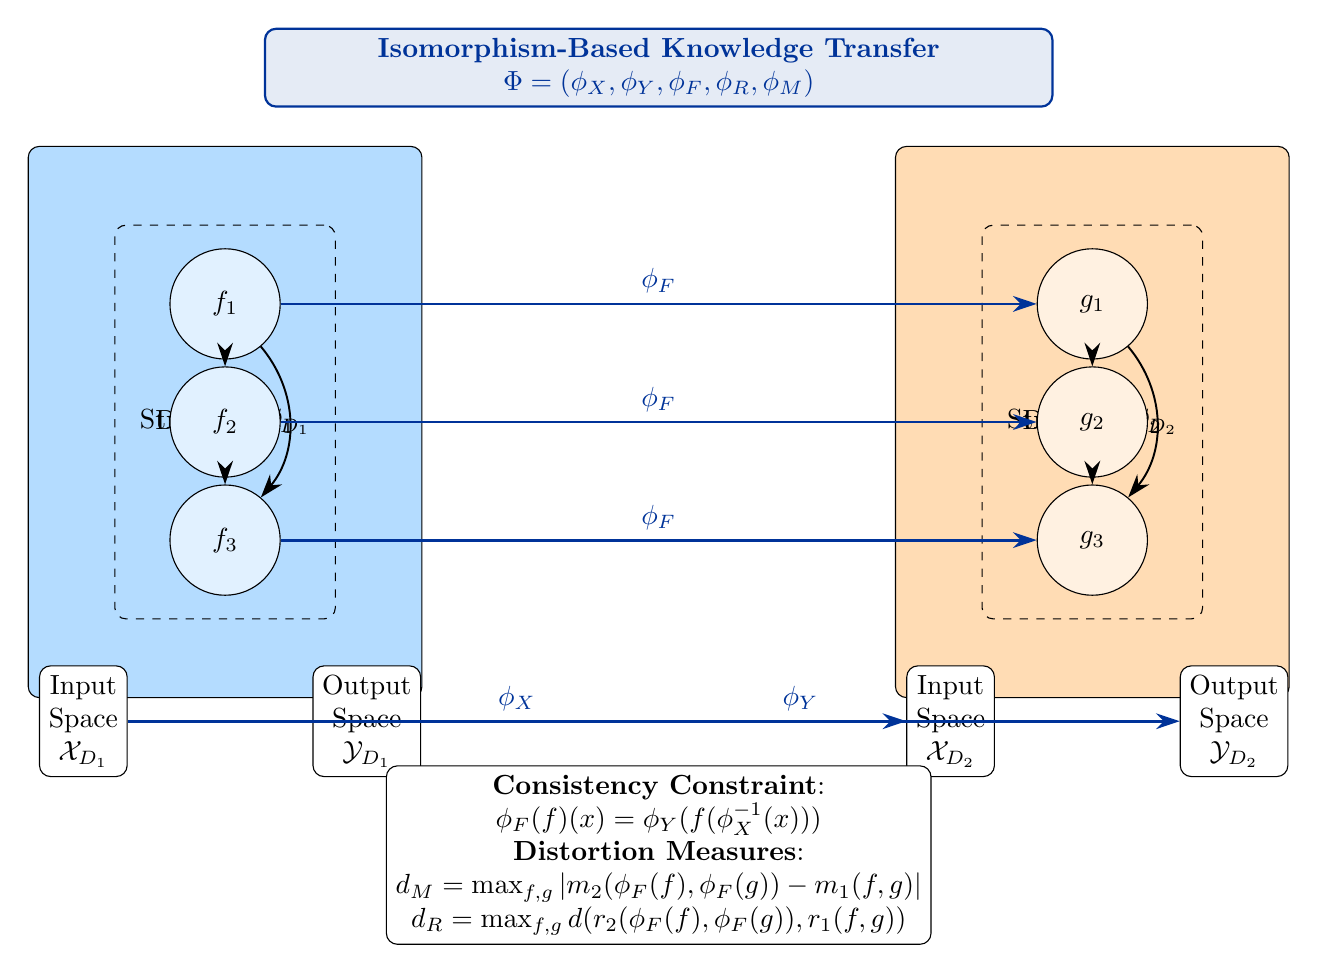
\begin{tikzpicture}[
    node distance=2.5cm,
    knowledge/.style={circle, draw, fill=white, minimum size=1.4cm, align=center},
    structure/.style={draw, dashed, rounded corners, minimum width=2.8cm, minimum height=5cm, align=center},
    domain1/.style={draw, fill=domain1, rounded corners, minimum width=5cm, minimum height=7cm, align=center},
    domain2/.style={draw, fill=domain2, rounded corners, minimum width=5cm, minimum height=7cm, align=center},
    arrow/.style={-{Stealth[length=3mm, width=2mm]}, line width=0.7pt},
    iso/.style={-{Stealth[length=3mm, width=2mm]}, DarkSkyBlue, line width=1pt},
    dasharrow/.style={dashed, ->, line width=0.5pt}
]

% Domains
\node[domain1] (d1) {Domain $D_1$};
\node[domain2, right=6cm of d1] (d2) {Domain $D_2$};

% Knowledge structures
\node[structure] (s1) at ($(d1) + (0,0)$) {Structure $S_{D_1}$};
\node[structure] (s2) at ($(d2) + (0,0)$) {Structure $S_{D_2}$};

% Knowledge in domain 1
\node[knowledge, fill=domain1!40!white] (k11) at ($(s1) + (0,1.5)$) {$f_1$};
\node[knowledge, fill=domain1!40!white] (k12) at ($(s1) + (0,0)$) {$f_2$};
\node[knowledge, fill=domain1!40!white] (k13) at ($(s1) + (0,-1.5)$) {$f_3$};

% Knowledge in domain 2
\node[knowledge, fill=domain2!40!white] (k21) at ($(s2) + (0,1.5)$) {$g_1$};
\node[knowledge, fill=domain2!40!white] (k22) at ($(s2) + (0,0)$) {$g_2$};
\node[knowledge, fill=domain2!40!white] (k23) at ($(s2) + (0,-1.5)$) {$g_3$};

% Relationships in domain 1
\draw[arrow] (k11) -- (k12);
\draw[arrow] (k12) -- (k13);
\draw[arrow, bend left=40] (k11) to (k13);

% Relationships in domain 2
\draw[arrow] (k21) -- (k22);
\draw[arrow] (k22) -- (k23);
\draw[arrow, bend left=40] (k21) to (k23);

% Isomorphism mapping
\draw[iso] (k11) -- (k21) node[midway, above, text=DarkSkyBlue] {$\phi_F$};
\draw[iso] (k12) -- (k22) node[midway, above, text=DarkSkyBlue] {$\phi_F$};
\draw[iso] (k13) -- (k23) node[midway, above, text=DarkSkyBlue] {$\phi_F$};

% Input/output spaces
\node[draw, fill=white, rounded corners, align=center] (x1) at ($(d1) + (-1.8,-3.8)$) {Input\\Space\\$\mathcal{X}_{D_1}$};
\node[draw, fill=white, rounded corners, align=center] (y1) at ($(d1) + (1.8,-3.8)$) {Output\\Space\\$\mathcal{Y}_{D_1}$};

\node[draw, fill=white, rounded corners, align=center] (x2) at ($(d2) + (-1.8,-3.8)$) {Input\\Space\\$\mathcal{X}_{D_2}$};
\node[draw, fill=white, rounded corners, align=center] (y2) at ($(d2) + (1.8,-3.8)$) {Output\\Space\\$\mathcal{Y}_{D_2}$};

% Space mappings
\draw[iso] (x1) -- (x2) node[midway, above, text=DarkSkyBlue] {$\phi_X$};
\draw[iso] (y1) -- (y2) node[midway, above, text=DarkSkyBlue] {$\phi_Y$};

% Title
\node[rectangle, draw, DarkSkyBlue, thick, rounded corners, fill=white!90!DarkSkyBlue, minimum width=10cm, align=center] 
    at ($(d1)!0.5!(d2) + (0,4.5)$) {
    \textbf{Isomorphism-Based Knowledge Transfer}\\
    $\Phi = (\phi_X, \phi_Y, \phi_F, \phi_R, \phi_M)$
};

% Consistency constraint
\node[rectangle, draw, rounded corners, fill=white, align=center] 
    at ($(d1)!0.5!(d2) + (0,-5.5)$) {
    \textbf{Consistency Constraint}:\\
    $\phi_F(f)(x) = \phi_Y(f(\phi_X^{-1}(x)))$\\
    \textbf{Distortion Measures}:\\
    $d_M = \max_{f,g} |m_2(\phi_F(f), \phi_F(g)) - m_1(f, g)|$\\
    $d_R = \max_{f,g} d(r_2(\phi_F(f), \phi_F(g)), r_1(f, g))$
};

\end{tikzpicture}

\end{document}